%----------------------------------------------------------------------------------------
%    PACKAGES AND THEMES
%----------------------------------------------------------------------------------------

\documentclass[aspectratio=169,xcolor=dvipsnames]{beamer}
\usetheme{SimpleDarkBlue}

\usepackage{hyperref}
\usepackage{graphicx} % Allows including images
\usepackage{booktabs} % Allows the use of \toprule, \midrule and \bottomrule in tables

%----------------------------------------------------------------------------------------
%    TITLE PAGE
%----------------------------------------------------------------------------------------

\title{Hamiltonian Simulation}
\subtitle{Quantum Computing}

\author{Álvaro Sánchez-Paniagua, Ana Vargas, Gonzalo, Íñigo, Miguel Laredo}

\institute
{
    Based on the notes from Ashley Montaro % Your institution for the title page
}
\date{\today} % Date, can be changed to a custom date

%----------------------------------------------------------------------------------------
%    PRESENTATION SLIDES
%----------------------------------------------------------------------------------------

\begin{document}

\begin{frame}
    % Print the title page as the first slide
    \titlepage
\end{frame}

\begin{frame}{Motivation}
\end{frame}


\begin{frame}{Overview}
    % Throughout your presentation, if you choose to use \section{} and \subsection{} commands, these will automatically be printed on this slide as an overview of your presentation
    \tableofcontents
\end{frame}





%%%%%%%%%%%%%%%%%%%
% Ana
%%%%%%%%%%%%%%%%%%%

\section{Introduction}
\begin{frame}{Introduction: Hamiltonian \textcolor{lightgray}{Simulation}}
    \begin{block}{Hamiltonian}
        Hermitian operator acting on $n$ qubits which corresponds physically to a system made up of $n$ 2-level subsystems.
    \end{block}
    \begin{block}{Schrödinger’s equation}
        Time evolution of the state $|\psi\rangle$ of a quantum system:
        \begin{align*}
            i \hbar \frac{d}{dt}|\psi(t)\rangle = H(t)|\psi(t)\rangle
        \end{align*}
    \end{block}
\end{frame}

\begin{frame}{Introduction: \textcolor{lightgray}{Hamiltonian} Simulation}
    Solution of the Schrödinger’s equation (\textit{time-independent}):
    \begin{align*}
        |\psi(t)\rangle = e^{-iHt}|\psi(0)\rangle
    \end{align*}
    \begin{block}{Goal}
        To approximate the unitary operator:
        \begin{align*}
            U(t) =  e^{-iHt}
        \end{align*}
    \end{block}
    Approximation in the operator (spectral) norm:
    \begin{align*}
        ||A|| := \max_{|\psi\rangle \neq 0}\frac{||A|\psi\rangle||}{|||\psi\rangle||}.
    \end{align*}
    $\~{U}$ approximates $U$ within $\epsilon$ if
        \begin{align*}
            ||\~{U} - U|| < \epsilon
        \end{align*}
\end{frame}


%%%%%%%%%%%%%%%%%%%
% Alvaro
%%%%%%%%%%%%%%%%%%%

%%%%%%%%%%%%%%%%%%%
% Miguel
%%%%%%%%%%%%%%%%%%%

\begin{frame}{Hamiltonian as a Pauli Matrix Product}
  We consider the simple case where $H$ is proportional to a Pauli matrix on $n$ qubits:
  \begin{equation}
    H = \alpha s_1 \otimes s_2 \otimes \cdots \otimes s_n.
  \end{equation}
  The corresponding time evolution operator is:
  \begin{equation}
    e^{-i t H} = e^{-i t \alpha s_1 \otimes s_2 \otimes \cdots \otimes s_n}.
  \end{equation}
  \textbf{Challenge:} $H$ is a $2^n \times 2^n$ matrix with exponentially many parameters, but we seek a circuit of poly$(n)$ gates.
\end{frame}

\begin{frame}{Diagonalization of the Evolution Operator}
  Using the identity:
  \begin{equation}
    U e^{-i \alpha H} U^{\dagger} = e^{-i \alpha U H U^{\dagger}},
  \end{equation}
  we diagonalize $e^{-i t H}$ with an appropriate unitary transformation:
  \begin{equation}
    e^{-i t H} = (U_1 \otimes U_2 \otimes \cdots \otimes U_n) e^{-i \alpha t z_1 \otimes z_2 \otimes \cdots \otimes z_n} (U_1^{\dagger} \otimes U_2^{\dagger} \otimes \cdots \otimes U_n^{\dagger}),
  \end{equation}
  where $z_i \in \{I, Z\}$.
\end{frame}

\begin{frame}{Implementation via Quantum Circuits}
  The main challenge reduces to implementing:
  \begin{equation}
    e^{-i \alpha t Z \otimes Z \otimes \cdots \otimes Z}.
  \end{equation}
  For computational basis state $\ket{x}$:
  \begin{equation}
    \ket{x} \mapsto \begin{cases} 
      e^{-i\alpha t} \ket{x}, & \sum_i x_i \text{ even}, \\
      e^{i\alpha t} \ket{x}, & \sum_i x_i \text{ odd}.
    \end{cases}
  \end{equation}
  \textbf{Solution:} A quantum circuit using 2-qubit gates.
\end{frame}

\begin{frame}{Quantum Circuit for $k=4$}
  \begin{center}
    \begin{figure}[htbp]
      \centering
      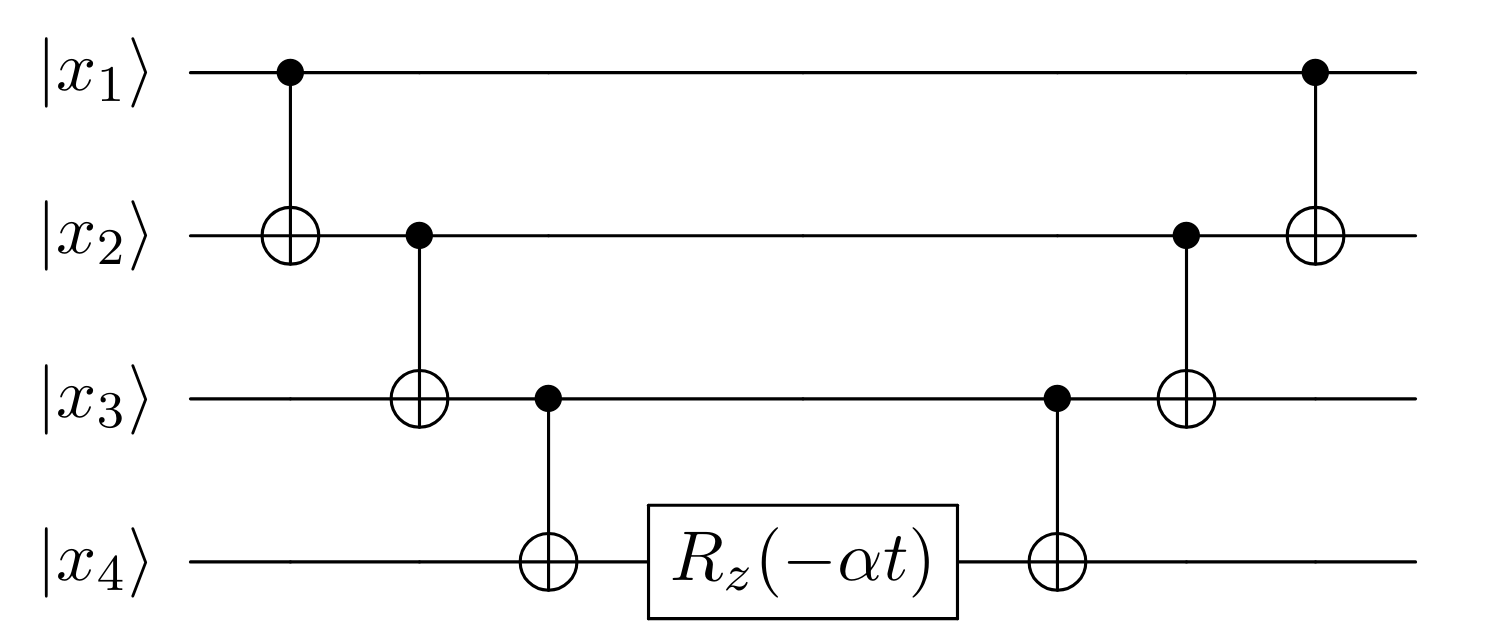
\includegraphics[width=0.8\textwidth]{rsc/circuit.png}
    \end{figure}

  \end{center}
  $R_z(\theta) = \begin{bmatrix} e^{i \theta} & 0 \\ 0 & e^{-i \theta} \end{bmatrix}$
\end{frame}

\begin{frame}{Generalization to Weighted Sums of Pauli Matrices}
  For $H$ as a weighted sum of commuting Pauli matrices:
  \begin{equation}
    H = \sum_{j=1}^{m} \alpha_j \sigma_{s_j},
  \end{equation}
  the evolution follows as:
  \begin{equation}
    e^{-i H t} = \prod_{j=1}^{m} e^{-i \alpha_j \sigma_{s_j} t}.
  \end{equation}
  This requires $O(mn)$ quantum gates.
\end{frame}

%%%%%%%%%%%%%%%%%%%
% Gonzalo
%%%%%%%%%%%%%%%%%%%

%%%%%%%%%%%%%%%%%%%
% Inigo
%%%%%%%%%%%%%%%%%%%


\end{document}
